\documentclass[12pt]{article}
%Gummi|065|=)
\usepackage{amsmath, amsfonts, amssymb}
\usepackage[margin=0.5in]{geometry}
\usepackage{xcolor}
\usepackage{graphicx}
\newcommand{\off}[1]{}
\DeclareMathSizes{20}{30}{21}{18}



\newcommand{\myhrule}{}

\usepackage{tikz}

\title{\textbf{ An Inversion Problem }}
\author{John D Mangual}
\date{}
\begin{document}

\fontfamily{qag}\selectfont \fontsize{24}{30}\selectfont

\maketitle

\noindent I ask around for a solution to an inversion problem.  Everyone could show me \textbf{how} to solve it but nobody wanted put the solution\footnote{I didn't ask ``how would you solve it" -- I was asking for an explicity answer, with a center and a radius.  Nobody wanted to.  If you do it neatly takes about a page (or less).  If you don't know algebra it takes 10 pages and you get nowhere.  This was a skill in textbook in 19th century -- and in fact all of my resources come from that time period.} \\ 
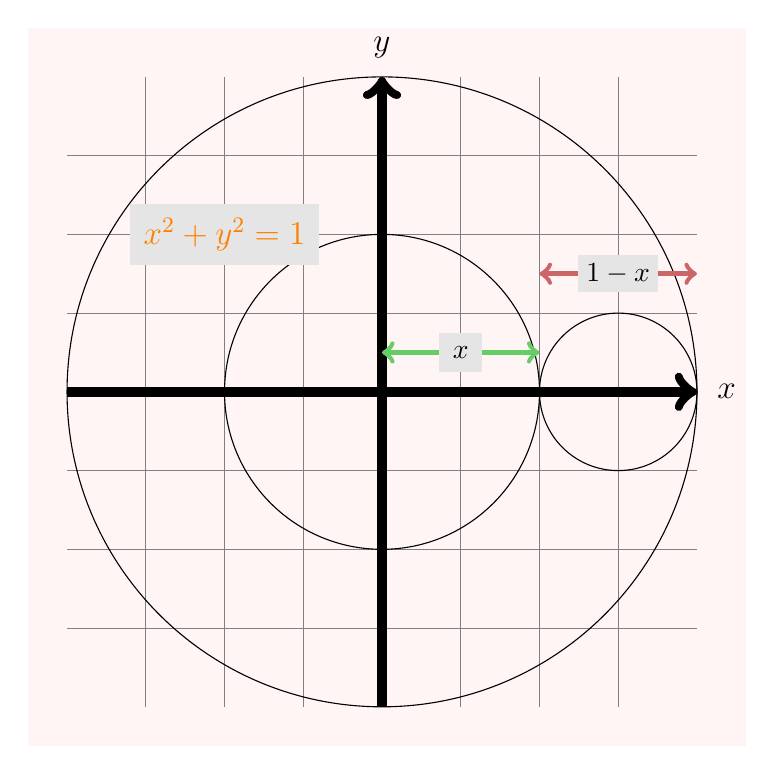
\begin{tikzpicture}

\fill[color=red!4!white] (-4.5,-4.5)--(-4.5,4.625)--(4.625,4.625)--(4.625,-4.5)--cycle;

\foreach \x in {-3,...,3}
	{
		\draw[color=black!50!white] (\x,-4)--(\x,4);
		\draw[color=black!50!white] (-4,\x)--(4,\x);
	}
	
\draw[->, line width=0.05in] (-4,0)--(4,0);
\draw[->, line width=0.05in] (0,-4)--(0,4);

\draw (0,0) circle (4);
\draw (0,0) circle (2);
\draw (3,0) circle (1);

\draw [<->, line width=0.025in, color=green!50!white!80!black] (0,0.5)--(2,0.5);

\node[fill=black!10!white, inner sep=5pt] at  (1,0.5) {\normalsize $x$} ; 

\draw [<->, line width=0.025in, color=red!50!white!80!black] (2,1.5)--(4,1.5);

\node[fill=black!10!white, inner sep=3pt] at  (3,1.5) {\normalsize $1-x$} ; 

\node[fill=black!10!white, inner sep=5pt] at (-2,2) {\color{orange}{\large $ {x^2 + y^2 = 1}$}};

\node at (4.375, 0) {\large $x$};

\node at (0, 4.375) {\large $y$};

\end{tikzpicture} \\ 
Let $a = \frac{1}{3}$.  I would like the image of these circles under the map:
$$ z \mapsto \frac{z - a}{\overline{a}z-1} $$


\newpage

\noindent \textbf{A} - the Easy Way \\ \\
This particular layout of circle is symmetric about the $x$ axis --- so we might\footnote{The small circle $|z-3|=\frac{1}{4}$ is moving in between $|z|=1$ and the image of $|z|=\frac{1}{2}$.  What happens (under inversion) if I rotate this figure? My question is what the image of the circle is under the map $z \mapsto  \frac{z - a}{\overline{a}z-1} $ and also $a = e^{i\theta} \frac{1}{3}$ and $\theta \in [0, 2\pi]$. } find an easier solution!


\newpage

\noindent \textbf{B} - from Old Textbooks


\newpage

\fontfamily{qag}\selectfont \fontsize{12}{10}\selectfont

\begin{thebibliography}{}

\item Curtis McMullen.  \textbf{Uniformly Diophantine Fixed Numbers in a Real Quadratic Field}

\item Jean Bourgain, Alex Kontorovich.
\textbf{Beyond Expansion II: Traces of Thin Semigroups} \texttt{arXiv:1310.7190v1}

\end{thebibliography}


\end{document}